\chapter{Ontologias}
\label{chap:ontologias}

\lettrine{A}{} palavra Ontologia veio do grego, assim como vários outros termos que se referem a alguma área de estudo. Seu significado, no entanto, é muito mais abstrato. Diferentemente de Biologia, que é "o estudo da vida", a palavra cujo plural dá nome a este capítulo quer dizer "o estudo do ser enquanto ser". O dicionário Merriam-Webster \footnote{\url{http://www.merriam-webster.com}} estende essa definição como: "um ramo da metafísica preocupado com a natureza e as relações do ser".

Importado da Filosofia, esse conceito começa a ser trabalhado muito antes da época dos computadores. Aristóteles já estudava Ontologia em suas Categorias \citep{ontoDahlberg}. No entanto, apenas em 1606, com o livro \textit{Ogdoas Scholastica}, de Jacob Lorhard, foi que a palavra em si realmente surgiu. Esse termo ficou popular em 1729 com o livro \textit{Philosophia Prima: sive Ontologia}, de Christian Wolff, com a definição "\textit{Ontology or First Philosophy is the science of Being in general or as Being}" \footnote{"Ontologia ou Filosofia Primeira é a ciência do ser em real ou como um ser."}  \citep{ontoNickles}.

Para a Ciência da Computação, a definição é um pouco diferente, embora possua muita semelhança com o conceito já explícito. Guarino definiu ontologia como "um artefato de engenharia, constituído por um vocabulário específico usado para descrever uma certa realidade, mais uma série de pressupostos explícitos acerca do significado que se atribui a esse vocabulário" \citep{ontoGuarino}. Logo, uma ontologia é uma reunião de sentenças lógicas que exibem alguma informação sobre alguma área do mundo para resolver algum problema relacionado a ela.

Fazendo um paralelo entre ambas as disciplinas, pode-se observar que, enquanto a primeira faz um estudo sistemático da existência, na segunda existe um foco maior no que pode ser representado.

As ontologias são estudadas na área de Inteligência Artificial, que está preocupada com a automação do comportamento inteligente. Na prática, elas funcionam como um sistema ''\textit{tell and ask}'' \cite{ontoRussel}. Algumas coisas são contadas para os agentes inteligentes (uma entidade autônoma com comportamento que simula inteligência), e então, perguntas podem ser feitas para eles, embora não precisem saber todas as respostas. 

Surgiram de um contexto onde os cientistas desejam modelar e representar o mundo para as máquinas, e isso ocorre desde a origem dos computadores. Como cada pessoa possui uma visão de mundo, cada modelagem será diferente de algum jeito. Por isso, a construção de ontologias é um tópico que merece estudo.

As ontologias denotam uma "especificação explícita de uma conceitualização"  \citep{ontoGruber}, e, uma vez construídas, permitem comunicação, compartilhamento e reúso de conhecimentos.

\section{Conceitualização}
	
Existe um certo debate sobre a definição de Conceitualização. Depois de propor o que era uma ontologia, Gruber sugeriu que uma Conceitualização "é uma visão abstrata e simplificada do mundo que se quer representar para algum propósito". Essa definição parece boa, mas deixa algumas pontas soltas. O que seria uma "visão", por exemplo, deixa algumas dúvidas.

Para Guarino e Giaretta, uma Conceitualização pode ser entendida como “uma estrutura semântica intensional que codifica as regras implícitas que determinam a estrutura de uma porção da realidade” \citep{ontoGiaretta}. Essa definição é um pouco mais concreta, e já é possível pensar sobre ela computacionalmente.

Pode-se inferir que uma Conceitualização é uma modelagem de parte de algum domínio do conhecimento. O domínio nada mais seria do que alguma disciplina, como a Geografia, Música, Enologia, entre outros. Tal modelagem é feita a partir de alguma linguagem formal de representação (em geral, Lógicas de Descrição) e deve levar em conta a generalidade que se aplica ao domínio escolhido.

Vale lembrar que, embora sejam amplamente utilizadas na vida real, as linguagens naturais (como a língua portuguesa e a lingua inglesa) não são consideradas linguagens formais. Isso tem uma explicação simples. Basta lembrar das figuras de linguagem, como a metáfora e o eufemismo, amplamente usadas nos discursos escrito e falado. 

\section{Construindo uma ontologia}

Para construir uma ontologia, é necessário escolher um domínio e o nível de generalidade que é necessário que ela atinja. Também deve-se ter em mente quem vai usá-la. Para que ela alcance o máximo de utilidade, é necessário que as perguntas que se deseja que ela responda sejam feitas antes de sua construção.

Geralmente, grandes ontologias são projetadas por equipes interdisciplinares, para que ela seja o mais correta e abrangente quanto possível. Quando se confecciona uma Ontologia, é necessário que sejam feitas algumas decisões de projeto.  

Gruber fez uma proposta de critérios de \textit{design} para ontologias com o objetivo de tornar o compartilhamento de conhecimento e interoperabilidade com programas baseados em conhecimento mais fácil \citep{ontoGruber}. Eles são os seguintes:

\begin{description}
	\item[Clareza] Uma ontologia deve ter uma linguagem clara e efetiva na definição de seus termos. Tal definição deve ser objetiva. Embora ela possa vir de situações sociais ou requisitos computacionais, ela deve ser independente destes contextos. Usar uma linguagem lógica, é um meio para este fim, ou seja, quando for possível fazer uma definição usando axiomas lógicos, isso deve ser feito. Onde possível, uma definição completa (com condições necessárias e suficientes) é preferível a uma definição parcial (com condições necessárias ou suficientes). Todas devem ser documentadas usando linguagem natural.
	\item[Coesão] Uma ontologia deve permitir inferências consistentes com suas definições. No mínimo, os axiomas usados nas definições devem ser logicamente consistentes. A coerência também deve ser aplicada aos conceitos informais, definidos na linguagem natural da documentação e nos exemplos. Se uma sentença que pode ser inferida contradiz uma definição ou exemplo dado informalmente, a ontologia não é coesa.
	\item[Estendibilidade] Uma ontologia deve ser projetada para ser capaz de antecipar o uso de conhecimento compartilhado. Ela deve oferecer uma fundação conceitual de modo que o novo conhecimento possa ser apoiado nela e que a ontologia possa ser estendida e especializada, ou seja, novos termos podem ser definidos usando o vocabulário existente, de modo que a revisão das crenças do conhecimento anterior possa ser evitada ao máximo.
	\item[Viés mínimo de codificação] A Conceitualização deve ser especificada num nível de conhecimento que não dependa de uma codificação que utiliza um nível de símbolos particulares. Um viés de codificação ocorre quando as escolhas de representação são feitas por pura conveniência de notação ou de implementação. Como agentes de conhecimento podem ser implementados em diferentes sistemas e estilos de representação, isso deve ser minimizado.
	\item[Compromisso ontológico mínimo] Isso faz com que ela suporte as atividades de compartilhamento de conhecimento desejadas. Quanto menos suposições sobre o mundo modelado, melhor. Isso permite que as partes comprometidas com a ontologia sejam livres para especializar e instanciar a ontologia o quanto quiserem. Já que isso é baseado no uso consistente do vocabulário, ele pode ser minimizado usando uma teoria fraca (genérica) e definindo apenas os conceitos necessários para a comunicação do conhecimento consistente com esta teoria.
\end{description}

É possível notar que todos esses critérios poderão não ser atendidos ao mesmo tempo, portanto, alguns \textit{trade-offs} deverão ser feitos.
Podemos ter um conflito, por exemplo, entre os critérios \textbf{Clareza} e \textbf{Estendibilidade}, já que o máximo de clareza implica que as definições terão a sua interpretação restrita.

\subsection{Componentes de uma ontologia}

Computacionalmente falando, as ontologias possuem cinco partes. Para ilustrá-las melhor, vamos fazer uma ontologia sobre Música. Será usada uma fonte monoespaçada para as partes dela.

\begin{description}
	\item[Classes] Descrevem os conceitos de um certo domínio do discurso. São o foco das ontologias. São uma coleção de todos os particulares aos quais é possível aplicar um termo geral. Por exemplo: a classe \texttt{Cantor}.
	\item[Propriedades] São atributos que descrevem características do conceito a que uma classe se refere. Em nosso exemplo, a classe \texttt{Cantor} possui as propriedades \texttt{Nome}, \\ \texttt{RitmoPredominante} e \texttt{Idade}.
	\item[Relações] Ontologias são constituídas de relações hierárquicas. Por exemplo \texttt{Cantor} $ \to $ \texttt{Pes\-so\-a}. A hierarquia de classes representa uma relação “\textit{is-a}” \citep{ontoFranca}. Tais relações são transitivas. Existem outras relações, como \texttt{Cantor canta Musica} e \texttt{Compositor compoe Musica}.
	\item[Restrições] São os tipos das propriedades, por exemplo: enquanto para \texttt{Nome} e \\ \texttt{RitmoPredominante} uma \textit{string} seja suficiente, para a Idade, um inteiro já está de bom tamanho. Além disso, as restrições podem ser referentes às classes. Exemplo: a releção \texttt{canta} tem domínio \texttt{Cantor.}
	\item[Instância] é um indivíduo (por exemplo, \texttt{MariahCarey}), de uma classe (como \texttt{Cantor}, \texttt{Com\-po\-si\-tor} ou \texttt{Pessoa}). Vale lembrar que uma instância não é uma subclasse.
\end{description}

Uma classe pode ter nomes diferentes em certo idiomas (por exemplo, \texttt{Cantor} e \texttt{Singer} seriam a mesma classe). Isso não é um problema pois não é o nome que define uma classe. Sinônimos e palavras em línguas distintas não representam classes diferentes.

Várias classes subordinadas a uma superclasse são consideradas irmãs. Elas devem ter o mesmo nível de generalidade. Por exemplo, seja uma classe \texttt{Musica}. Suas subclasses podem ser \texttt{Cancao}, \texttt{MusicaArgentina} e \texttt{MusicaBrasileira}. Tais classes são irmãs.

Existem três processos para definir as classes e a hierarquia, a seguir:

\begin{description}
	\item[\textit{Top-down}] Vai das classes mais genéricas para as mais específicas. Um exemplo seria criar as classes \texttt{Musica}, \texttt{Pessoa}, entre outras.
	\item[\textit{Bottom-up}] Vai das classes mais específicas para as mais genéricas, agrupando as específicas já criadas. Na ontologia estudada aqui, é possível começar das músicas já conhecidas para então separá-las por ritmos.
	\item[Vai-e-Vem] Define conceitos simples para generalizá-los e especificá-los. É uma com\-bi\-na\-ção dos dois primeiros itens.
\end{description}

\subsection{Montando a ontologia}

Montar uma ontologia é um processo que segue os seguintes passos:

\begin{itemize}
	\item Definir as classes da ontologia.
	\item Colocá-las em uma hierarquia taxonômica.
	\item Determinar suas propriedades e restrições.
	\item Criar uma base de conhecimento para essas classes e propriedades, ou seja, preencher a ontologia com as instâncias.
	\item Colocar os valores das propriedades para as instâncias.
\end{itemize}

Embora pareça ser direto, esse processo é iterativo, como afirmam Noy e McGuinness  \citep{ontoNoy}. Uma vez feito, deve ser repetido para que haja uma adequação das classes com as instâncias colocadas, pois, por exemplo, se uma classe acabar com apenas uma subclasse, a modelagem pode ter um problema, ou a ontologia não está completa. E ainda, se uma classe possui mais de uma dúzia de subclasses, novas categorias (classes ou subclasses) podem ser necessárias. 

Às vezes, uma classe possui muitas propriedades específicas e diferentes em várias de suas instâncias. Nesse caso, a inserção de uma classe deixará a ontologia mais compreensível. A nova classe fará com que a distinção das instâncias ocorra, efetivamente, evitando mal-entendidos.

Teoricamente, o processo nunca acaba. Na prática, ele é interrompido quando a ontologia fornece respostas suficientemente boas para a maior parte das consultas realizadas, ou seja, tal critério é subjetivo.

Ainda em relação às classes, algumas observações podem ser feitas. A primeira é em relação à herança múltipla. Ela acontece quando uma classe é subclasse de várias outras classes, por exemplo, a classe \texttt{PopBrasileiro}, pode pertencer à classe \texttt{Pop} e à classe \texttt{MusicaBrasileira}. Isso é aceitável, pois no mundo real, acontece várias vezes e de diversas maneiras.

As ontologias podem representar classes disjuntas. Classes disjuntas são aquelas que não possuem uma intersecção. Em nossa ontologia, \texttt{Cantor} e \texttt{Compositor} não são disjuntas. No entanto, \texttt{Cancao} e \texttt{HinoNacional} são classes disjuntas.

Para os nomes das classes, não há uma convenção específica, só há um consenso de que manter um padrão de nomenclatura é algo bom. Para fazer isso, pode-se usar \texttt{snake\textunderscore case}, \texttt{camelCase} ou usar espaços na grafia.

Uma ontologia não precisa ter toda a informação existente sobre o domínio. Não é necessário especializar ou generalizar mais do que seja necessário para a aplicação. Além disso, as classes não precisam ter todas as propriedades possíveis e nem carregar todas as distinções que estão no mundo. Isso significa que a ontologia deve ser o modelo mais simples para o problema que se deseja resolver.

Algumas relações podem ter uma inversa, assim como ocorre com funções matemáticas. Uma relação que possui uma inversa pode ser \texttt{Cantor canta Musica}, com sua inversa sendo \texttt{Musica cantadaPor Cantor}.

\section{Usabilidade de uma ontologia}

A criação de uma ontologia é feita por uma equipe interdisciplinar, geralmente composta por \textit{experts} da área que se deseja cobrir e técnicos para a confecção de ontologias (vindos da área de Computação). Isso não impede a equipe de possuir profissionais de mais áreas. Uma ontologia é feita para que qualquer pessoa possa acessar suas informações.

Ontologias feitas sobre áreas de estudo (por exemplo, a Aviação) são muito mais úteis do que aquelas feitas sobre acontecimentos (como a queda do voo TAM 3054). A existência dessa última nem faz sentido, já que as ontologias servem para modelar casos gerais, não particulares. É melhor, por exemplo, construir uma ontologia sobre acidentes de avião e seus conceitos.

\section{Problemas relacionados}

Existem alguns problemas relacionados a ontologias. Os mais comuns são os problemas de modelagem e construção. Um problema muito comum é a existência, na linguagem natural, de Homônimos e Sinônimos. Deve existir um cuidado especial com eles, já que eles podem levar a uma confusão na nomenclatura.

Em relação à modelagem, o problema de não utilizar uma equipe interdisciplinar especializada pode levar a uma cobertura incompatível de conceitos, ou seja, as classes podem ficar muito distantes da realidade. Além disso, usar fontes não confiáveis na ontologia pode fazer com que os problemas que elas estavam sendo feitas para resolver, não sejam resolvidos corretamente.

Tais problemas tornam-se muito maiores quando duas ontologias são integradas. A possível integração entre ontologias é um dos motivos para elas existirem, afinal, isso pode acelerar o seu desenvolvimento. Em nosso exemplo, se já existir uma ontologia sobre Música Brasileira, poderemos absorvê-la, mas o cuidado terá de ser redobrado em relação às questões acima. 

Em relação à implementação, os pontos que surgem são em geral a respeito da linguagem utilizada, mas isso será tratado no \autoref{chap:logicas}.

Além dos já citados, pode acontecer de chegar um novo conhecimento e a ontologia ficar inconsistente. Neste caso, terão de ser usadas algumas operações de Revisão de Crenças, foco deste trabalho, que será estudado no \autoref{chap:revisao}.

A ontologia desenvolvida nesse capítulo segue na Figura \ref{img:Esquema}

\begin{figure}
	\centering
	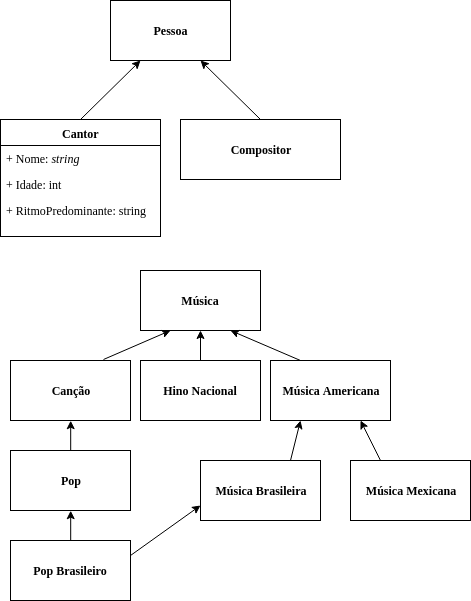
\includegraphics[width=0.6\textwidth]{Capitulos/Ontologias/OntologiaMusica}
	\caption{Esquema de classes de uma ontologia sobre Música}
	\label{img:Esquema}
\end{figure}